% Created 2026-03-05 Thu 13:56
% Intended LaTeX compiler: pdflatex
\documentclass[11pt]{article}
\usepackage[utf8]{inputenc}
\usepackage[T1]{fontenc}
\usepackage{graphicx}
\usepackage{longtable}
\usepackage{wrapfig}
\usepackage{rotating}
\usepackage[normalem]{ulem}
\usepackage{amsmath}
\usepackage{amssymb}
\usepackage{capt-of}
\usepackage{hyperref}
\usepackage{minted}
\author{arunneru}
\date{\today}
\title{}
\hypersetup{
 pdfauthor={arunneru},
 pdftitle={},
 pdfkeywords={},
 pdfsubject={},
 pdfcreator={Emacs 31.0.50 (Org mode 9.7.11)}, 
 pdflang={English}}
\begin{document}

\tableofcontents

\section{Cusp bifurcation}
\label{sec:org1f58783}

\begin{equation}
\dot{x} = \mu + \lambda x - x^{3}
\end{equation}


\begin{minted}[]{python}
from auto import *
import numpy as np
import matplotlib.pyplot as plt
\end{minted}



\begin{minted}[]{bash}
ls | grep cusp
\end{minted}

\begin{center}
\begin{tabular}{llllll}
c.cusp & cusp.auto & cusp.exe & cusp.f90 & cusp.ipynb & cusp.o\\
\end{tabular}
\end{center}


\begin{minted}[]{python}
cusp = load('cusp')
mu = run(cusp)
mu = mu + run(cusp, DS='-')

mu = rl(mu)
save(mu, 'mu')
lp1 = load(mu('LP1'), ISW=2)


\end{minted}



\begin{minted}[]{python}
plt.plot(mu[0]['x'],mu[0]['mu'], 'k')
plt.plot(mu[1]['x'],mu[1]['mu'], 'r')
plt.savefig("./images/cubic_xVsmu.png", format="png")
plt.show()
plt.close()
\end{minted}


\begin{figure}[htbp]
\centering
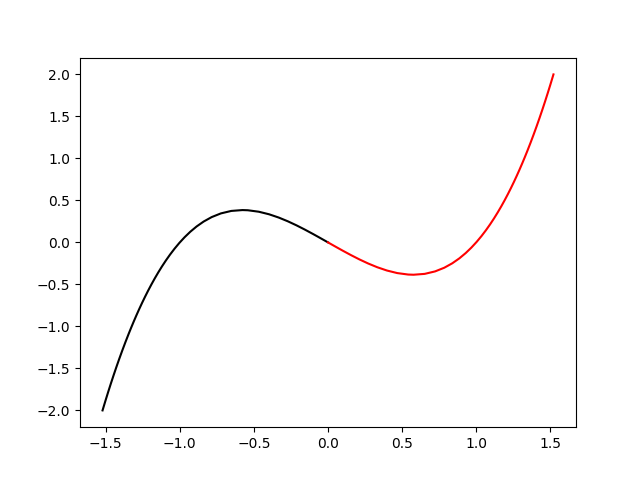
\includegraphics[width=.9\linewidth]{./images/cubic_xVsmu.png}
\caption{\label{fig:orgc5c96f2}The cubic shaped x-nullcline as a function of the parameter \(\mu\)}
\end{figure}


\begin{minted}[]{python}
mu.summary()
\end{minted}


\begin{verbatim}

BR    PT  TY  LAB       mu         L2-NORM          x           lambda    
 1     1  EP    1   0.00000E+00   0.00000E+00   0.00000E+00   1.00000E+00
 1    14  LP    2   3.84900E-01   5.77360E-01  -5.77360E-01   1.00000E+00
 1    20        3   1.26582E-01   9.29410E-01  -9.29410E-01   1.00000E+00
 1    40        4  -1.38347E+00   1.40803E+00  -1.40803E+00   1.00000E+00
 1    47  UZ    5  -1.99999E+00   1.52138E+00  -1.52138E+00   1.00000E+00

BR    PT  TY  LAB       mu         L2-NORM          x           lambda    
 1     1  EP    6   0.00000E+00   0.00000E+00   0.00000E+00   1.00000E+00
 1    14  LP    7  -3.84900E-01   5.77360E-01   5.77360E-01   1.00000E+00
 1    20        8  -1.26582E-01   9.29410E-01   9.29410E-01   1.00000E+00
 1    40        9   1.38347E+00   1.40803E+00   1.40803E+00   1.00000E+00
 1    47  UZ   10   1.99999E+00   1.52138E+00   1.52138E+00   1.00000E+00
\end{verbatim}


\begin{verbatim}

BR    PT  TY  LAB       mu         L2-NORM          x           lambda    
 1     1  EP    1   0.00000E+00   0.00000E+00   0.00000E+00   1.00000E+00
 1    14  LP    2   3.84900E-01   5.77360E-01  -5.77360E-01   1.00000E+00
 1    20        3   1.26582E-01   9.29410E-01  -9.29410E-01   1.00000E+00
 1    40        4  -1.38347E+00   1.40803E+00  -1.40803E+00   1.00000E+00
 1    47  UZ    5  -1.99999E+00   1.52138E+00  -1.52138E+00   1.00000E+00

BR    PT  TY  LAB       mu         L2-NORM          x           lambda    
 1     1  EP    6   0.00000E+00   0.00000E+00   0.00000E+00   1.00000E+00
 1    14  LP    7  -3.84900E-01   5.77360E-01   5.77360E-01   1.00000E+00
 1    20        8  -1.26582E-01   9.29410E-01   9.29410E-01   1.00000E+00
 1    40        9   1.38347E+00   1.40803E+00   1.40803E+00   1.00000E+00
 1    47  UZ   10   1.99999E+00   1.52138E+00   1.52138E+00   1.00000E+00
\end{verbatim}


\begin{minted}[]{python}
lp1
\end{minted}


\begin{verbatim}
  BR    PT  TY  LAB ISW NTST NCOL NDIM IPS IPRIV
   1    14  LP    2   1    1    0    1   1     0
Pointset cusp (parameterized)
Independent variable:
t:  [0.]
Coordinates:
x:  [-0.57735966]
Labels by index: Empty
Active ICP: [2]
rldot: [np.float64(0.0018853769549)]
udotps: Pointset cusp (non-parameterized)
Coordinates:
UDOT(1):  [-0.99999822]
Labels by index: Empty
PAR(1:5):       lambda             mu                 PAR(3)             PAR(4)             PAR(5)         
              1.0000000000E+000  3.8490017931E-001  0.0000000000E+000  0.0000000000E+000  0.0000000000E+000
PAR(6:10):    0.0000000000E+000  0.0000000000E+000  0.0000000000E+000  0.0000000000E+000  0.0000000000E+000
PAR(11:11):   0.0000000000E+000
\end{verbatim}


\begin{verbatim}
  BR    PT  TY  LAB ISW NTST NCOL NDIM IPS IPRIV
   1    14  LP    2   1    1    0    1   1     0
Pointset cusp (parameterized)
Independent variable:
t:  [0.]
Coordinates:
x:  [-0.57735966]
Labels by index: Empty
Active ICP: [2]
rldot: [np.float64(0.0018853769549)]
udotps: Pointset cusp (non-parameterized)
Coordinates:
UDOT(1):  [-0.99999822]
Labels by index: Empty
PAR(1:5):       lambda             mu                 PAR(3)             PAR(4)             PAR(5)         
              1.0000000000E+000  3.8490017931E-001  0.0000000000E+000  0.0000000000E+000  0.0000000000E+000
PAR(6:10):    0.0000000000E+000  0.0000000000E+000  0.0000000000E+000  0.0000000000E+000  0.0000000000E+000
PAR(11:11):   0.0000000000E+000
\end{verbatim}

\begin{minted}[]{python}
cusp = run(lp1)
cusp = cusp + run(lp1, DS='-')
save(cusp, 'cusp')
\end{minted}


\begin{minted}[]{python}
cusp.summary()
\end{minted}


\begin{verbatim}

BR    PT  TY  LAB       mu         L2-NORM          x           lambda    
 2    20       11   1.09209E+00   8.17354E-01  -8.17354E-01   2.00420E+00
 2    34  UZ   12   1.99995E+00   9.99991E-01  -9.99991E-01   2.99995E+00

BR    PT  TY  LAB       mu         L2-NORM          x           lambda    
 2    20       11   5.42543E-02   3.00470E-01  -3.00470E-01   2.70847E-01
 2    29  CP   12  -2.02770E-12   1.00472E-04   1.00472E-04   3.02839E-08
 2    40       13  -9.09414E-02   3.56925E-01   3.56925E-01   3.82187E-01
 2    60       14  -5.73716E-01   6.59512E-01   6.59512E-01   1.30487E+00
 2    80       15  -1.68023E+00   9.43582E-01   9.43582E-01   2.67104E+00
 2    85  UZ   16  -1.99995E+00   9.99992E-01   9.99992E-01   2.99995E+00
\end{verbatim}


\begin{verbatim}

BR    PT  TY  LAB       mu         L2-NORM          x           lambda    
 2    20       11   1.09209E+00   8.17354E-01  -8.17354E-01   2.00420E+00
 2    34  UZ   12   1.99995E+00   9.99991E-01  -9.99991E-01   2.99995E+00

BR    PT  TY  LAB       mu         L2-NORM          x           lambda    
 2    20       11   5.42543E-02   3.00470E-01  -3.00470E-01   2.70847E-01
 2    29  CP   12  -2.02770E-12   1.00472E-04   1.00472E-04   3.02839E-08
 2    40       13  -9.09414E-02   3.56925E-01   3.56925E-01   3.82187E-01
 2    60       14  -5.73716E-01   6.59512E-01   6.59512E-01   1.30487E+00
 2    80       15  -1.68023E+00   9.43582E-01   9.43582E-01   2.67104E+00
 2    85  UZ   16  -1.99995E+00   9.99992E-01   9.99992E-01   2.99995E+00
\end{verbatim}



\begin{minted}[]{python}
import matplotlib.pyplot as plt

plt.plot(cusp[0]['mu'], cusp[0]['lambda'])
plt.plot(cusp[1]['mu'], cusp[1]['lambda'])
plt.savefig("./images/bifurcation_diagram_cusp.png")
plt.show()
plt.close()
\end{minted}

\begin{figure}[htbp]
\centering
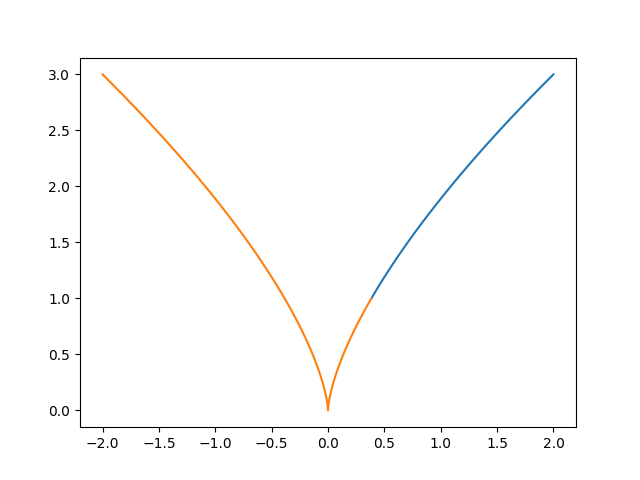
\includegraphics[width=.9\linewidth]{./images/bifurcation_diagram_cusp.png}
\caption{\label{fig:orgff9e92e}The bifurcation diagram showing the evolution of the saddle-node point in the \(\mu-\lambda\) plane}
\end{figure}
\end{document}
